%~~~~~~~~~~~~~~~~~~~~~~~~~~~~~~~~~~~~~~~~~~~~~~~~~~~~~~~~~~~~~~~~~~~~~~~
\section{Conceitos Básicos}\label{sec:concepts}
%~~~~~~~~~~~~~~~~~~~~~~~~~~~~~~~~~~~~~~~~~~~~~~~~~~~~~~~~~~~~~~~~~~~~~~~

A fim facilitar o entendimento dos conceitos explorados nos próximos capítulos, introduzimos aqui os conceitos básicos utilizados ao longo deste trabalho.

Em especial, abordaremos alguns conceitos básicos de probabilidade, explicando desde o conceito de espaço amostral até variáveis aleatórias e estimadores; conceitos essenciais para explicar e demonstrar as propriedades de estruturas de dados probabilísticas. 

Além disso, faremos uma revisão do estado da arte sobre funções \emph{hash} e modelos de fluxo de dados, que serão bastante referenciados ao longo deste trabalho.

\subsection{Introdução à probabilidade}

O assunto estruturas de dados probabilísticas claramente depende muito da teoria e notações da cálculo de probabilidades. Neste trabalho, a fim de facilitar o entendimento, introduzimos o assunto utilizando notação definida em \cite{figueiredo2007randomizados}.

\subsubsection{Espaço probabilístico}

Define-se o \emph{espaço probabilístico} como formado por dois componentes: um \emph{espaço amostral} $\Omega = \{r_1, r_2, \cdots\}$, que representa os possíveis resultados de um experimento aleatório, e uma \emph{função de probabilidade} $\Pr$, que define a probabilidade com que qualquer \emph{evento} $A \subseteq \Omega$ ocorre em experimentos aleatórios. Esta função precisa respeitar as seguintes propriedades:

\begin{enumerate}
  \item Para todo evento $A \subseteq \Omega$, $0 \leq \Pr[A] \leq 1$.
  \item $\Pr[\Omega] = 1$.
  \item Para eventos $A_1, A_2, ..., A_n$ disjuntos, $\Pr[\bigcup_i A_i] = \sum_i \Pr[A_i]$.
\end{enumerate}

No caso de eventos $A_1, A_2, ..., A_n$ arbitrários (isto é, não necessariamente disjuntos), vale o \emph{princípio da inclusão-exclusão}:
\begin{alignat*}{2}
    \Pr\left[ \bigcup_i A_i \right] = & \sum_i \Pr[A_i] \\
                                  & - \sum_{i<j} \Pr[A_i \cap A_j] \\
                                  & + \sum_{i<j<k} \Pr[A_i \cap A_j \cap A_k] \\
                                  & - \cdots \\
                                  & + (-1)^{l+1} \sum_{i_1 < i_2 < \cdots < i_l} \Pr \left[ \bigcap_{r=1}^{l} A_{i_r} \right] \\
                                  & + \cdots
\end{alignat*}
e em especial
\[
    \Pr[A_1 \cup A_2] = \Pr[A_1] + \Pr[A_2] - \Pr[A_1 \cap A_2]
\]

Como exemplo destes conceitos, podemos analisar as probabilidades envolvidas no lançamento de um dado de seis lados. Definimos $\Omega = \{1, 2, 3, 4, 5, 6\}$, representando todos os possíveis resultados deste experimento. 

Sabemos que a probabilidade de qualquer resultado $E_i = \{r_i\}, r_i \in \Omega$ é igual, isto é $\Pr[E_i] = {^{1}/_{6}}$. Podemos calcular que a probabilidade de um lançamento resultar em 2 ou 5 é dada pela probabilidade da união entre os dois eventos que, para conjuntos disjuntos, é igual a: $\Pr[\{2, 5\}] = \Pr[\{2\}] + \Pr[\{5\}] = {^2/_6} = {^1/_3}$.

Entretanto, para calcular a probabilidade do resultado ser um número divisível por dois (evento \textsc{Div2}) ou por três (evento \textsc{Div3}) podemos utilizar o princípio da inclusão-exclusão. Assim 
\[
\Pr[\textsc{Div2} \cup \textsc{Div3}] = \Pr[\textsc{Div2}] + \Pr[\textsc{Div3}] - \Pr[\textsc{Div2} \cap \textsc{Div3}]
\]
ou seja,
\begin{alignat*}{2}
\Pr[\{2,4,6\} \cup \{3,6\}] &= \Pr[\{2,4,6\}] + \Pr[\{3,6\}] - \Pr[\{6\}] \\
                            &= {^3/_6} + {^2/_6} - {^1/_6} \\
                            &= {^4/_6}
\end{alignat*}

\subsubsection{Variáveis aleatórias}

Uma \emph{variável aleatória} $X$ é uma função que mapeia o espaço amostral em um outro conjunto. Neste trabalho apenas lidaremos com variáveis aleatórias reais, na forma $X : \Omega \to \mathbb{R}$. 

A função \emph{densidade de probabilidade} de uma variável aleatória real é definida como $p_X(x) : \mathbb{R} \to [0, 1]$. $p_X(x) = \Pr[X = x]$, que é outra forma de escrever $\Pr[\{r \in \Omega \mid X(r) = x\}]$, ou seja, a probabilidade do resultado $r$ de um experimento aleatório seja tal que $X(r) = x$.

O valor esperado (ou esperança) de uma variável aleatória consiste na média de todos os possíveis valores que ela pode assumir, ponderada pela probabilidade que cada valor tem de ser assumido. Isto é,
\[
    \text{E}[X] = \sum_{x \in \mathbb{R}} x p_X(x).
\]

Por exemplo, considere o resultado do lançamento de dois dados de seis lados. Podemos definir a variável $X$ como a soma dos valores obtidos nos dados. Assim, temos por exemplo que $p_X(3) = {^2/_{36}}$, pois apenas dois resultados possíveis neste experimento resultam na soma 3 ($1+2$ e $2+1$). Por outro lado, $p_X(7) = {^6/_{36}}$, pois seis resultados possíveis no espaço amostral somam 7 ($1+6$, $2+5$, etc.). Assim, o valor esperado para a variável $X$ é:
\begin{align*}
    \text{E}[X] &= 2 \cdot p_X(2) + 3 \cdot p_X(3) + ... + 12 \cdot p_X(12) \\
          &= 2 \cdot {^1/_{36}} + 3 \cdot {^2/_{36}} + ... + 12 \cdot {^1/_{36}} \\
          &= 7
\end{align*}

A \emph{linearidade da esperança} é a propriedade que diz que, para variáveis aleatórias $X_1, X_2, \cdots, X_n$ e uma função linear $h$, vale:
\[
    \text{E}[h(X_1, X_2, \cdots, X_n)] = h(\text{E}[X_1], \text{E}[X_2], \cdots, \text{E}[X_n])
\]

Ainda utilizando o exemplo do lançamento de dois dados, uma outra forma de calcular o valor esperado seria fazê-lo para apenas um dado e dobrar o resultado. Considere as variáveis aleatórias $Y_1$ e $Y_2$ como os valores resultantes do lançamento de cada um dos dados, tal que $X = Y_1 + Y_2$. Assim, pela linearidade da esperança, $\text{E}[X] = \text{E}[Y_1 + Y_2] = \text{E}[Y_1] + \text{E}[Y_2]$. 

O valor esperado para $Y_i$ é mais fácil de calcular, sendo apenas a média simples entre todos os resultados possíveis no lançamento de um dado:
\[
    \text{E}[Y_i] = \frac{1+2+3+4+5+6}{6} = \frac{21}{6} = \frac{7}{2}
\]
logo
\[
    \text{E}[X] = \text{E}[Y_1] + \text{E}[Y_2]  = \frac{7}{2} + \frac{7}{2} = 7
\]

Uma propriedade importante de variáveis aleatórias é sua variância, que pode ser definda da seguinte forma:
\[
    \text{Var}[X] = \text{E}[(X - \text{E}[X])^2] = \text{E}[X^2] - (\text{E}[X])^2
\]

Dadas variáveis aleatórias independentes $X_1, X_2, \cdots, X_n$, todas com a mesma variância $\sigma^2$, a \emph{fórmula de Bienaymé} reza sobre a variância da média $\bar{X}$ dessas variáveis:
\[
    \text{Var}[\bar{X}] = \text{Var}\left[ \frac{1}{n} \sum_{i=1}^{n} X_i \right] = \frac{1}{n^2} \sum_{i=1}^{n} \text{Var}[X_i]  = \frac{\sigma^2}{n}
\]

Isto significa, na prática, que a média entre $n$ variáveis independentes diminui a variância por um fator de $n$. Este resultado é útil para estruturas de dados probabilísticas, pois permite diminuir o erro compondo estimadores independentes.

Algumas variáveis aleatórias são muito comumente vistas na teoria e possuem muitas propriedades já estudadas. Para este trabalho iremos focar na variável de \emph{Bernoulli} e na variável \emph{binomial}, sendo a primeira apenas um caso especial da segunda.

A variável de Bernoulli pode assumir apenas dois valores: 0 ou 1. Ela representa o resultado de um experimento onde o valor 0 representa um "fracasso" e o valor 1 um "sucesso". Seja $p$ a probabilidade de sucesso, temos que
\[
    p_X(x) = \begin{cases}
        1 - p  & \text{se } x = 0 \\
        p      & \text{se } x = 1 \\
        0      & \text{para demais valores de } x \\
        
    \end{cases}
\]

É fácil demonstrar que para uma variável de Bernoulli $X$, $\text{E}[X] = p$ e $\text{Var}[X] = p (1-p)$.

A variável binomial representa o total de sucessos em uma série de $n$ experimentos e pode ser vista como o somatório de $n$ variáveis de Bernoulli com uma mesma probabilidade $p$.

Denota-se $B(n, p)$ a variável binomial que representa o total de sucessos de $n$ experimentos com probabilidade $p$. A densidade de probabilidade desta variável é
\[
    p_{B(n,p)} = \begin{cases}
        {\binom{n}{x}} p^x(1-p)^{n-x}    & \text{para } 0 \leq x \leq n \\
        0                               & \text{para demais valores de x} \\
    \end{cases}
\]

O valor esperado da variável binomial pode ser inferido pela linearidade da esperança de cada variável de Bernoulli que a compõem, ou seja $E[B(n, p)] = np$. 

A partir da definição $\text{E}[X^2] = n (n-1) p^2 + np$, podemos calcular a variância da variável binomial: $\text{Var}[X] = np(1-p)$.

Perceba que a variável de Bernoulli é apenas um caso especial de uma variável binomial, $B(1, p)$.

\subsubsection{Desigualdades probabilísticas}

Embora o valor esperado de uma variável aleatória nos forneça valiosa informação sobre como uma variável se comporta na média de vários experimentos, ele não nos diz muito sobre a distribuição dos valores que a variável pode assumir.

Ao utilizar estruturas de dados probabilísticas, por exemplo, calculamos o valor de variáveis aleatórias cujo valor esperado é igual ao que se deseja estimar. Entretanto, para ter alguma utilidade prática, é preciso poder prever a probabilidade de erro.

A seguir apresentaremos algumas desigualdades que permitem definir um limite superior na probabilidade da variável aleatória assumir certos intervalos de valores.

A \emph{desigualdade de Markov}, por exemplo, diz que para variáveis $X$ que somente assumem valores não-negativos,
\[
    \Pr[X \geq a] \leq \frac{\text{E}[X]}{a} \text{, para todo } a > 0
\].

Se a variância da variável for conhecida, um limite mais forte pode ser estabelecido, através da \emph{desigualdade de Chebyshev}:
\[
    \Pr[|X - \text{E}[X]| \geq a] \leq \frac{\text{Var}[X]}{a^2} \text{, para todo } a > 0
\]

É possível reescrever esta desigualdade definindo o desvio padrão $\sigma = \sqrt{\text{Var}[X]}$. Assumindo $a = k\sigma$,
\[
    \Pr[|X - \text{E}[X]| \geq k\sigma] \leq \frac{1}{k^2} \text{, para todo } k > 1
\]

Este limite mostra, de forma intuitiva, como as probabilidades de cada um dos valores de $X$ se comportam conforme eles se afastam de $\text{E}[X]$.

Sem mais informações sobre a variável não é possível definir limites gerais mais fortes para sua distribuição. Entretanto, para alguns tipos de variáveis específicas é possível utilizar a \emph{desigualdade de Chernoff} para encontrar limites específicos desta distribuição. Existem diversas variantes desta desigualdade, cada uma específica para um tipo de variável aleatória. Em especial, abordaremos aqui o uso desta desigualdade para variáveis de Bernoulli.

Considere uma variável $X = \sum_{i=1}^n X_i$, onde todo $X_i$ é uma variável de Bernoulli independente com probabilidade $p_i$. Seja também $\mu = \text{E}[X] = \sum_{i=1}^n p_i$. Então, dois limites se aplicam:

\begin{itemize}
  \item \textbf{Limite superior:} $\Pr[X \geq (1 + \delta)\mu] \leq e^{-\frac{\delta^2}{2+\delta}\mu}$ para todo $\delta > 0$;
  \item \textbf{Limite inferior:} $\Pr[X \leq (1 - \delta)\mu] \leq e^{-\mu\delta^2/2}$ para todo $0 < \delta < 1$;
\end{itemize}

Uma versão simplificada que combina combina os dois limites é definida por
\[
    \Pr[|X - \mu| \geq \delta\mu] \geq 2e^{-\mu\delta^2/3}\text{ para todo } 0 < \delta < 1.
\]

\subsubsection{Estimadores}

Um estimador é uma regra que permite estimar um certo parâmetro $\theta$ de uma variável aleatória $X$ a partir de observações sobre a mesma. São funções denotadas $\hat{\theta} : E \to \Theta$, onde $E$ é o contra-domínio da variável $X$ e $\Theta$ é chamado de espaço paramétrico.

Estimadores também são variáveis aleatórias por si só, portanto possuem média, variância, desvio padrão etc.

O viés de um estimador é a diferença entre seu valor esperado e o parâmetro que ele almeja estimar, ou seja, $\text{B}(\hat{\theta}) = \text{E}[\hat{\theta}] - \theta$. Um estimador é considerado \emph{não-enviesado} se e somente se $\text{B}(\hat{\theta}) = 0$.

A variância de um estimador é um parâmetro importante para analisar seu erro padrão. A variância, assim como em uma variável aleatória, mede o quanto cada observação se afasta de seu valor valor esperado e é definida como:
\[
    \text{Var}[\hat{\theta}] = \text{E}[(\hat{\theta} - \text{E}[\hat{\theta}])^2] = \text{E}[\hat{\theta}^2] - (\text{E}[\hat{\theta}])^2
\]

Consequentemente, o erro padrão de um estimador é definido como $\sigma_{\hat{\theta}} = \sqrt{\text{Var}[\hat{\theta}}]$.

O erro médio quadrático (EMQ) de um estimador combina variância e viés em um único conceito. Em vez de comparar a diferença entre cada observação e o valor esperado do estimador, compara-se com o valor real do parâmetro. Isto é $\text{EMQ}[\hat{\theta}] = \text{E}[(\hat{\theta} - \theta)^2]$. Em um estimador não-enviesado, o EMQ é igual à variância.

\subsection{Funções \emph{hash}}

Todas as estruturas descritas neste trabalho são baseadas em funções \emph{hash} e são, de certa forma, dependentes das propriedades das funções utilizadas. Por isso, apresentamos aqui um breve resumo das características principais esperadas de funções aplicáveis a estruturas de dados probabilísticas.

O objetivo principal das funções \emph{hash} neste contexto é a capacidade de simular certa aleatoriedade a um conjunto de dados que pode ter um grau de entropia muito baixo. Como Knuth diz em \cite{knuth1998art}, é impossível definir uma função que cria dados aleatórios a partir de dados não aleatórios, mas na prática é possível criar uma imitação boa o suficiente.

\subsubsection{Tabelas \emph{hash}}

A aplicação mais direta de funções \emph{hash} é a possibilidade de mapear chaves contidas em conjuntos muito grandes a entradas numa tabela com tamanho potencialmente bem menor do que os conjuntos que representam, uma tabela \emph{hash}. Por exemplo, é possível mapear \emph{strings}, um conjunto infinito, para inteiros na tabela, de forma que a complexidade esperada para verificar sua existência seja independente do tamanho da tabela, e sim proporcional ao tamanho da \emph{string}. A Figura~\ref{fig:hashtable} mostra um exemplo deste tipo de tabela.

\begin{figure}[!htbp]
  \centering
  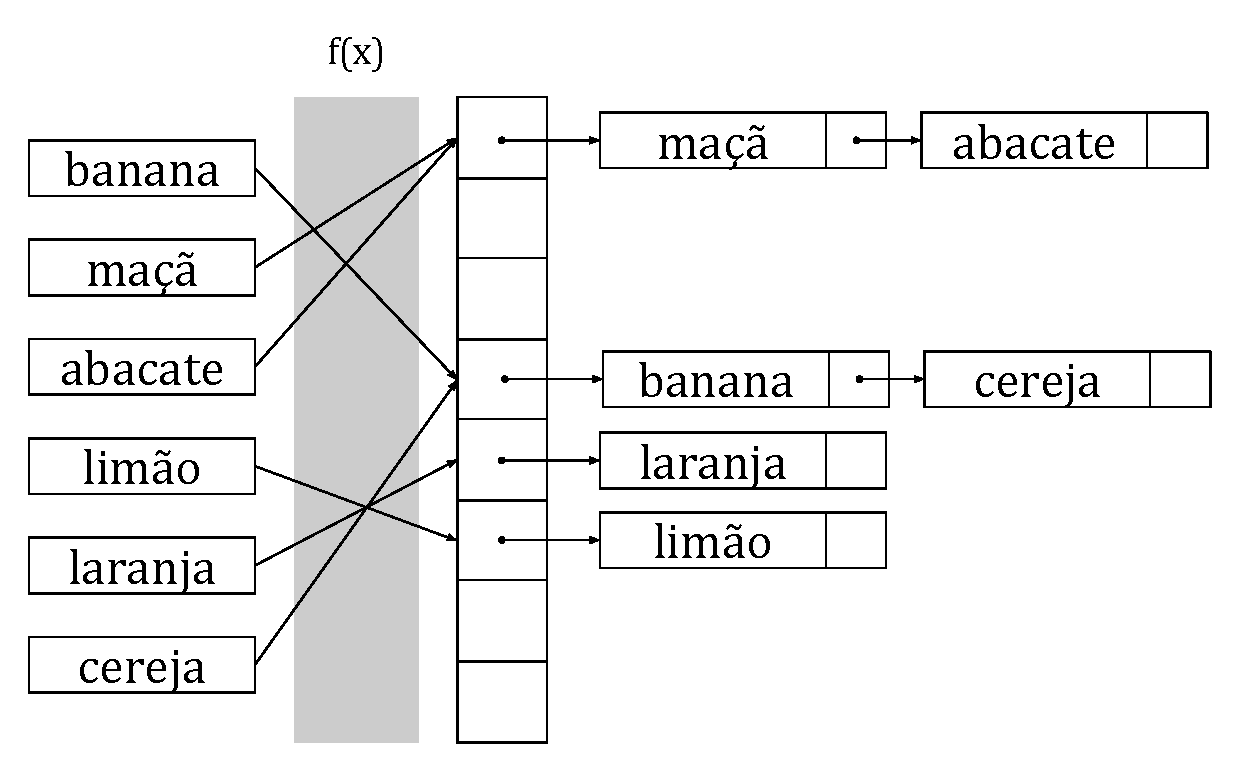
\includegraphics[scale=0.6]{files/hashtable.pdf}
  \caption{Exemplo de tabela \emph{hash}}
  \label{fig:hashtable}
\end{figure}

O exemplo dado assume algumas propriedades da função \emph{hash} escolhida, em especial:
\begin{itemize}
  \item \textbf{A distribuição da imagem é aparentemente uniforme:} isto é, a probabilidade aparente de qualquer um dos valores do contradomínio ser escolhido para representar a entrada é igual. Esta é uma propriedade impossível de alcançar na teoria e sua aplicação prática pode ser amplamente dependente do domínio da função, por exemplo: uma função \emph{hash} que funciona bem para palavras em português pode não funcionar tão bem para palavras em inglês.
  
  \item \textbf{A função tem baixa complexidade (linear, de preferência):} Funções com complexidades maiores podem tornar a inserção e busca na tabela inviáveis.
  
  \item \textbf{A função é determinística:} esta é uma propriedade redundante, se assumirmos a definição usual de \emph{função}, entretanto dado o contexto é importante explicitá-la, visto que uma função \emph{hash} que resulta em valores diferentes (se aplicada várias vezes à mesma entrada) não tem valor para busca em tabelas. Dito isto, os conceitos de funções pseudo-aleatórias e funções \emph{hash} possuem grande interseção teórica.
\end{itemize}

Há outros detalhes teóricos e de implementação de tabelas \emph{hash} que não serão tratados aqui (como a resolução de colisões por exemplo), por não dizerem tanto a respeito de funções \emph{hash} em si, que são o foco desta seção.

\subsubsection{\emph{Hashs} criptográficos}

Não há um conjunto ideal de propriedades de funções \emph{hash} que sirva a todos os propósitos possíveis. As propriedades ideais para uso em uma tabela \emph{hash} não são os mesmos para o uso em aplicações de segurança, por exemplo. Nestas, é usualmente requerido que um usuário malicioso seja (na prática) incapaz de criar chaves que sejam mapeadas para um valor específico do contradomínio da função. Isto é, deseja-se que a tarefa encontrar a função inversa da função \emph{hash} seja computacionalmente inviável.

\subsubsection{\emph{Hashing} universal e \emph{HashDOS}}

\subsubsection{Exemplos de funções \emph{hash}}



\subsection{Modelo de processamento em fluxos de dados}

